In order to effectively plan paths and coordinate actions, the agents must maintain information about the current states of the other agents. To accomplish this, a liveness check algorithm will be implemented in each agent. This algorithm is depicted in Figure \ref{fig:liveness_check}.
\begin{figure}[H]
    \centering
    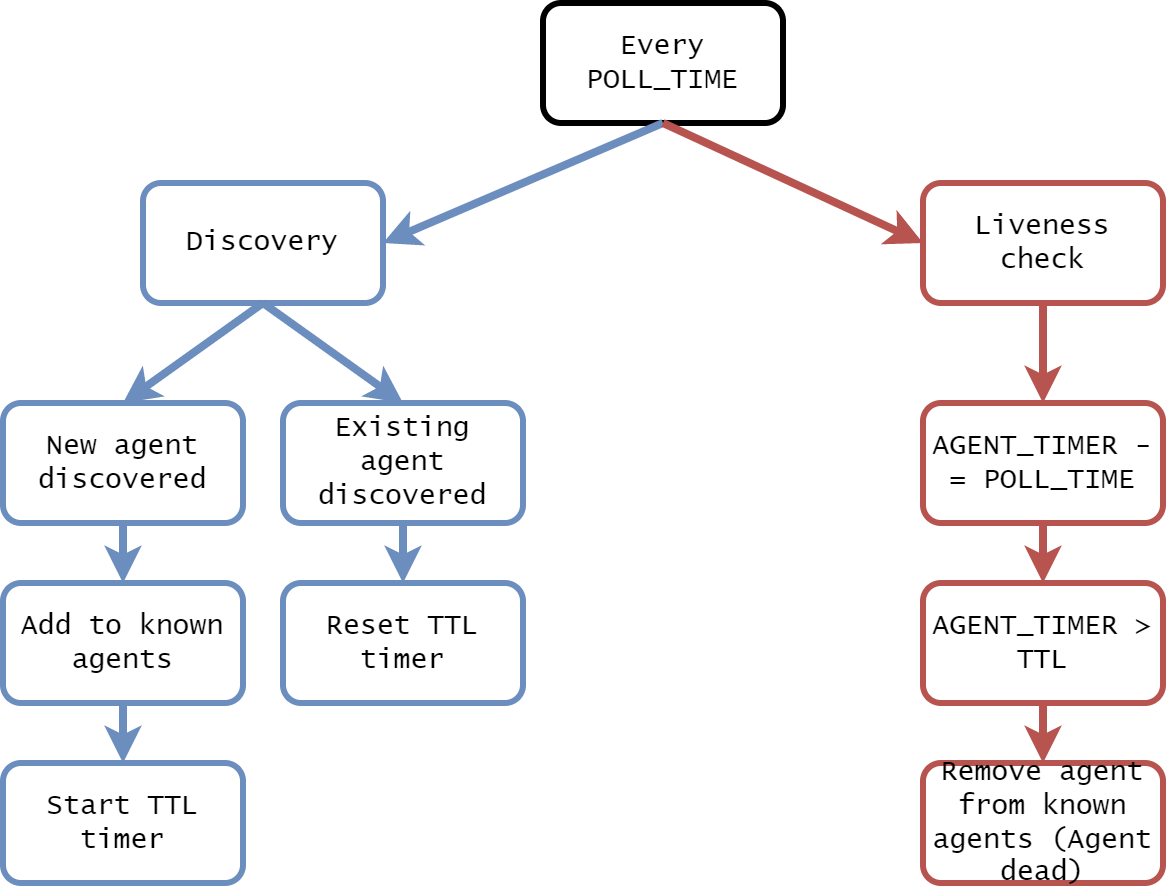
\includegraphics[width=0.8\textwidth]{pictures/agent_ttl.png}
    \caption{Liveness check}
    \label{fig:liveness_check}
\end{figure}

The liveness check algorithm is used to ensure that the agents maintain an accurate and up-to-date view of the states of the other agents in the system. The algorithm is executed periodically by each agent.

During each execution, the agent sends a discovery message to a specific topic, allowing other agents to discover it as a peer and marking it as alive. The agent also subscribes to the same topic to receive discovery messages from other agents. In the event that a new, unknown agent is discovered, it is added to the list of known agents and a Time-to-Live (TTL) timer is assigned and started for that agent. If the discovered agent is already known, the timer is simply restarted.

After sending the discovery message, the agent performs a liveness check by decrementing the timers of each known agent and checking if the timer exceeds the TTL. If the timer exceeds the TTL, it indicates that there have been no messages from that particular agent for a period longer than is allowed, and the agent is marked as dead. This allows the agent to maintain an accurate and up-to-date view of the states of the other agents in the system.
